\documentclass[UTF8]{article}

\usepackage{amsmath}
\usepackage[utf8]{inputenc}
\usepackage[OT4]{polski}
\usepackage{graphicx}
\usepackage{subcaption}
\usepackage{geometry}
\usepackage{titlesec}
\usepackage{graphicx}
\graphicspath{ {pics/} }

\geometry{left=2.5cm,right=2.5cm,top=2.5cm,bottom=2.5cm}
\titlelabel{\thetitle.\quad}

\title{%
	Sprawozdanie 1 \\
	\large Zadanie 24. Przedstaw liczbę 100 jako sumę dwóch liczb całkowitych dodatnich, których iloczyn jest maksymalny~}

\author{Adrian Rupala}


\begin{document}
\pagenumbering{gobble}
\maketitle

\newpage
\tableofcontents

\newpage
\pagenumbering{arabic}

\section{Teoria}

Każdy problem matematyczny należy rozpocząć od analizy treści pod kątem określenia sposobu rozwiązania. Zadanie to jest jednym z przykładów zadania optymalizacyjnego. Z treści wynika, że musimy odszukać pewne parametry, które są uwarunkowane inną zależną maksymalną. Schemat rozwiązania takich zadań wygląda następująco: ~

\begin{enumerate}
	\item Utworzenie równania bazującego na treści zadania (zależności parametrów do wartości podanej).
	\item Wyznaczenie wzoru funkcji $f(x)$ wynikającej z treści zadania. ~
	\item Obliczenie pochodnej funkcji $f(x)$,  którą stworzyliśmy. ~
	\item Obliczenie ekstremum funkcji $f(x)$. ~
	\item Wskazanie ekstremum, dla którego funkcja $f(x)$ osiąga szukaną wartość oraz w razie konieczności obliczenie drugiej szukanej wartości. ~
\end{enumerate}

\section{Rozwiązanie}

Z treści zadania wynika, że potrzebujemy zdefiniować dwie liczby naturalne dodanie, w przypadku tego rozwiązania zostały one zdefiniowane jako $x$ oraz $y$. Ich suma musi być równa $100$. Jesteśmy również w stanie za pomocą powstałego równania wyznaczyć jedną z wartości niewiadomych. ~
\\$x + y = 100 \Rightarrow y = 100 - x $\\
\\Kolejnym krokiem jest utworzenie funkcji, która będzie opisywała stosunek dwóch liczb, których iloczyn jest maksymalny, podstawienie do niego obliczonej wartości $y$, którą obliczyliśmy przekształcając powyższe równanie.~
\\$ f(x) = x \cdot y = x \cdot (100-x) = 100x - x^{2} $\\
\\Następnie, aby otrzymać wynik należy obliczyć pochodną funkcji pierwszego stopnia. Otrzymane w ten sposób równanie przyrównujemy do zera. ~
\\$ \frac{\partial}{\partial x}(100x - x^{2}) = 0$
\\$100 - 2x = 0$
\\$2x = 100$
\\$x = 50 $\\
\\W ten sposób obliczyliśmy wartość pierwszej szukanej przez nas liczby. Aby obliczyć kolejną wystarczy obliczoną liczbę wstawić do pierwszego wzoru opisującego stosunek dwóch liczb do liczby, jaką chcemy przedstawić.~
\\$ y = 50 - 100 \Rightarrow y = 50 $\\
\\W ten sposób obliczyliśmy poszukiwane przez nas dwie maksymalne liczby naturalne, których iloczyn jest maksymalny.~\\
\\Aby określić czy otrzymana przez nas liczba to maksimum lub minimum funkcji należy obliczyć miejsca, w których parabola przecina oś $x$ oraz narysować parabolę dla równania funkcji $100x - x^{2} = 0$ obliczonego wcześniej. ~\\
\\Wyciągając wspólny czynnik przed nawias otrzymamy równanie w postaci:~
\\$100x - x^{2} = 0 \Rightarrow -x(x-100)=0$\\
\\Następnie dzieląc obustronnie równanie przez $-1$:~
\\$x(x-100)=0$\\
\\Powyższe równanie zachodzi gdy:~
\\$x-100 = 0$ oraz $x=0$\\
\\Dodając $100$ obustronnie otrzymamy dwa miejsca, w których ramiona paraboli będą przecinały oś $x$:~
\\$x = 100$ oraz $x = 0$\\
\\Ramiona paraboli skierowane są w dół, ponieważ pierwszy współczynnik równania kwadratowego jest liczbą ujemną i wynosi $-1$. ~ 
\\Z rysunku 1 wynika, że punkt wierzchołka jest punktem najwyżej położonym, dlatego liczba $50$ jest lokalnym maksimum funkcji.~ 
\\Wykres funkcji wygląda następująco:~\\

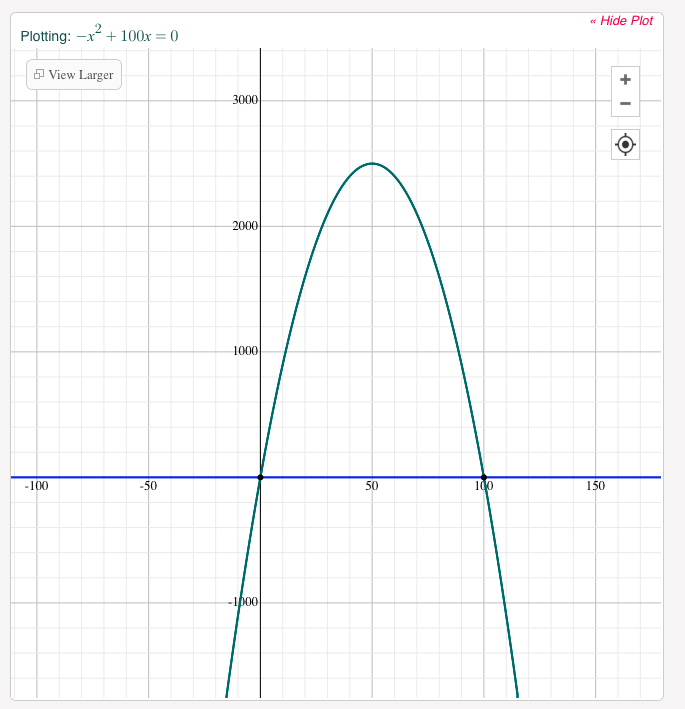
\includegraphics[width=10cm, height=10cm]{parab}\\
Rys. 1. Wykres funkcji $100x - x^{2} = 0$



\section{Odpowiedź}

	Szukane przez nas dwie wartości dla liczby $100$ to $x = 50$ oraz $y = 50$. ~

\end{document}